\documentclass[9pt,twocolumn,twoside]{../../styles/osajnl}
\usepackage{fancyvrb} \journal{i524}

\title{Oracle PGX}

\author[1,*]{Piyush Shinde}

\affil[1]{School of Informatics and Computing, Bloomington, IN 47408,
  U.S.A.}


\affil[*]{Corresponding authors: piyushsshinde1992@gmail.com}

\dates{project-001, \today}

\ociscodes{Graph Analysis, Algorithms, Shell}

% replace this with your url in github/gitlab
\doi{\url{https://github.com/cloudmesh/classes/blob/master/docs/source/format/report/report.pdf}}


\begin{abstract}
Graph analysis provides key insights that are normally overlooked when
glancing through them. These insights play a vital role in business
optimizations. Efficiency of graph analysis can be compromised due to
factors like storage capacity and data set sizes. Oracle PGX is a
graph analysis toolkit. This paper provides a brief introduction to
Oracle PGX and its various features. It also discusses the real world
applications, advantages and limitations.
\newline
\end{abstract}

\setboolean{displaycopyright}{true}

\begin{document}

\maketitle

\section{Introduction}

A graph is a fundamental data structure that defines links between
different entities (data). Graphs represent data sets in a wide range
of applications. In a social graph, for example, nodes correspond to
people while friendship relationships between them are represented as
edges \cite{hong2012green}.

Graph analysis involves extracting information from a data-set, which
is represented as a graph. Large amounts of data demands huge amounts
of computational power to analyse. Challenges faced during graph
analysis include storage capacity for large data sets, performance
variation with varying data set sizes, and efficient implementation of
graph analyses algorithms.

Oracle PGX (Parallel Graph AnalytiX) solves these challenges.  PGX is
a fast, parallel, in-memory graph analytic framework. Its main
features include loading graphs into memory, running built-in and
user-defined graph analyses algorithms, running graph pattern matching
queries and mutating graphs \cite{www-over}. We will glance through
these features in this paper.

\begin{figure}[h]
    \centering 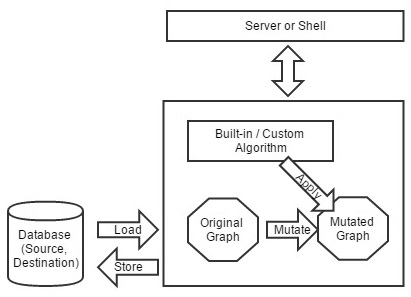
\includegraphics[scale=0.7]{images/1} \centering
    \caption{PGX Overview.}
    \end{figure}

\section{Installation}

To install Oracle PGX the platform requirements include a Linux x86
system (kernel >= 2.6) or Mac OS X platform \cite{www-plat}.

Oracle PGX can be installed in the following steps. Download Java SE 8
Development Kit (JDK8). Make sure the JAVA$\_$HOME environment
variable points to the JDK8 home directory, e.g. export
JAVA$\_$HOME=/usr/lib/jvm/java-8-oracle. Unzip the downloaded zip file
e.g. unzip pgx-2.3.1-server.zip -d /opt/pgx. Change directory (cd)
into the installation directory. e.g. cd $\$$PGX$\_$HOME. Start the
PGX shell using the command $./bin/pgx$.

Oracle PGX 2.3.1 is the latest version available as of $26^{th}$
February 2017 \cite{www-plat}.


\section{Usage Modes}
PGX provides four different usage modes, depending on different user
requirements \cite{www-usage}.

\subsection{Local Shell Mode}
This mode enables the user to interact with a PGX shell on a local
machine through a command-line shell interface. User commands are
dynamically interpreted and executed by the PGX shell to invoke the
PGX function. It can be used to run some quick graph analyses locally
on small graph data. It can likewise be used to try different graph
algorithms to explore the different interpretations of a data set.
    \begin{figure}[h]
    \centering 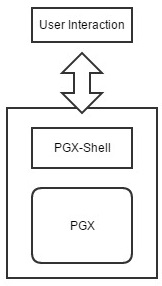
\includegraphics[scale=0.6]{images/2} \centering
    \caption{PGX Local Shell Mode.}
    \end{figure}
    
\subsection{Remote Shell Mode}
In the remote shell mode, the PGX execution engine is deployed as a
RESTful application on a powerful PGX-Server which is remotely
connected to the PGX-Shell from a client machine. This mode is useful
for performing graph analysis on large data sets. This mode enables to
connect multiple clients to the PGX-Server.
    \begin{figure}[h]
    \centering 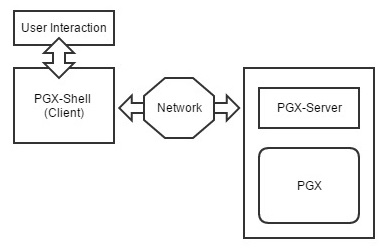
\includegraphics[scale=0.7]{images/3} \centering
    \caption{PGX Remote Shell Mode.}
    \end{figure}
    
\subsection{Local Java Application Mode}
This modes allows embedding PGX into a Java application, and using
graph analysis as a part of the application’s functionality.
    \begin{figure}[h]
    \centering 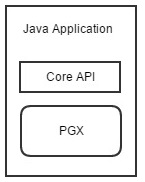
\includegraphics[scale=0.6]{images/4} \centering
    \caption{PGX Locally Embedded Mode.}
    \end{figure}
    
\subsection{Remote Java Application Mode}
This mode empowers the user to use the Java application to control the
PGX-Server remotely, from a client machine. Similar to the remote
shell model, this mode enables connections to the PGX-Server via
multiple clients.
    \begin{figure}[h]
    \centering 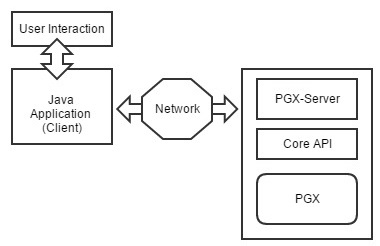
\includegraphics[scale=0.6]{images/5} \centering
    \caption{PGX Remotely Embedded Mode.}
    \end{figure}    

\section{Graph Mutations}
PGX helps users create mutated versions of the original graph, to
perform algorithms for graph analyses. Since PGX does not allow
mutation of the original graph, it always creates a new mutated
version of the original graph.

A graph can be simplified by removing self-edges, duplicated edges,
and trivial vertices.
    \begin{figure}[h]
    \centering 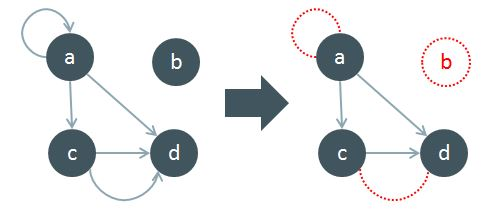
\includegraphics[scale=0.7]{images/6} \centering
    \caption{Simplifying a graph. Source: Paper \cite{www-mut}}
    \end{figure}
    
Graphs can also be simplified by undirecting it's edges. Subgraphs and
bipartite subgraphs can also be created in PGX.

\section{Running Graph Algorithms on PGX}
PGX allows you to run graph algorithms in two ways.

\textit{Built-in graphs:} PGX provides a set of built-in graph
algorithms that are ready to use. They include computing various
centrality measures, finding shortest paths, finding/evaluating
clusters and components, and predicting future edges, etc. The
detailed and complete list of the built-in algorithms, with their time
complexity, space requirement and implementation code is available on
the official website of Oracle Labs PGX.

\textit{Custom algorithms:} User-defined algorithms can be programmed
in PGX (excluding the ones from the built-in package), using the
Green-Marl language (a Domain Specific Language) \cite{www-graph}. The
Domain Specific Language approach provides benefits like productivity,
performance and portability.

\section{Use Cases}
PGX can be used to solve real world graph analyses problems. Here are
two such applications \cite{www-use}.

\subsection{Detect Potential Fraud in a Healthcare System}
In this example, anomalies in medical transactions were detected using
PGX.

A public data set of medical transactions from CMS (United States
Center for Medicare and Medicaid Services) for the year 2012 was
used. It had transactions between over 880,000 medical providers and
CMS, adding upto more than $\$$77B for 2012 \cite{www-hcs}.

To analyse the data, the data set was converted to a bipartite graph,
separating health care providers from health services. An edge in the
bipartite graph linked a specific health service to a health care
provider. A two-hop (undirected) path existed between two health care
providers, for each common health service they both provided. The more
common services between two health care providers, the closer they
would be to each other in the graph. The data set also specified the
‘specialities’ of medical providers. Vertices of medical providers of
the same speciality would be closer to each other, since they would
provide similar services. In case, a medical provider was
exceptionally close to other providers with different speciality, it
would be considered an anomaly since the medical provider would be
providing services unfitting to its speciality.

Personalized PageRanks (PPR) were used to compute closeness between
vertices. For each speciality a PPR score was computed. These scores
were then cross-checked to see if they belonged to the current
speciality. If not, the provider was considered an anomaly. This graph
analysis was implemented using the built in Personalized PageRank
algorithm.

The results were further investigated to identify potential frauds in
the Healthcare System.

\subsection{Using PGX as a Recommendation Engine}
This example helps us discover the information implied by
relationships through graph analytics.

A publicly available data set ‘MovieLens’ was used.  Recommendations
were generated using matrix factorization algorithm. Matrix
factorization is a simple process, in which you factorize a matrix
into two matrices, such that the newly generated matrices when
multiplied with each other would generate back the original matrix
\cite{www-rec}.

We had a matrix of movies and users, where the values were the ratings
given by the user to a movie. The aim was to recommend a bunch of
movies for each user.

An array of features was synthesized, considering user information,
the movies they rated and their ratings. The approach was to
initialize each matrix with some values. Each user had an array of
floating-point values that represented how strongly they were
associated with that feature. To generate recommendations, the movie’s
feature array was multiplied to the user’s feature array. The
corresponding values were then sorted in a descending fashion and the
top few items were the recommendations. This process was very fast
using PGX. The results were then used for many recommendations,
repeating the process periodically after new users or movies were
added to the system.


\section{Benefits and Limitations}
PGX executes graph algorithms in a fast, parallel, in-memory
fashion. It provides built-in algorithms and supports user-defined
algorithms. It offers an interleaved usage of graph analysis
algorithms and graph pattern-matching. In addition, it provides an
interactive shell application to easily execute commands from the
shell command line.

PGX loads file-systems, exclusively in graph formats. It requires
licensing, restricting its usage. Both of the above mentioned
limitations can be removed by contacting Oracle Labs PGX
\cite{www-limit}.

\section{Useful Resources}
The complete documentation of Oracle PGX, including instructions to
download and install and several tutorials, in a systematic method are
available on the main website of Oracle Labs PGX \cite{www-wel}.

The paper titled “Graph Analysis – Do We Have to Reinvent the Wheel?”,
discusses about the alternative database technologies that provide
optimized performance with regards to the dedicated graph
databases. \cite{welc2013graph}

The paper on Green-Marl DSL approach tilted "Green-Marl: A DSL for
Easy and Efficient Graph Analysis", provides insight on the methods of
using the Green-Marl DSL technique for optimizing graph analyses using
user-defined algorithms. \cite{hong2012green}

\section{Conclusion}
Numerous information is revealed from graphs. The analysis of graphs
can unveil significant insights. Oracle PGX (Parallel Graph AnalytiX)
is a toolkit for graph analysis. It allows users to load up their
graph data and run analytic algorithms on them. It provides different
usage modes which can be used as per client requirements. It allows
users to implement various built-in and user-defined graphs and mutate
graphs. Some classes of the built-in algorithms are community
detection, path finding, page ranking, recommendation, pattern
matching and influencer identification. Oracle PGX is easy to use. It
can be used for precise and efficient graph analysis, and is scalable
to implement graph analysis algorithms for large data sets.

\section{Acknowledgments}
This project was a part of the Big Data and Software and Projects
(INFO-I524) course. I would like to thank Professor Gregor von
Laszewski and the associate instructors for their help and support
during the course.

\bibliography{references}

\end{document}
